\documentclass[11pt]{preprint}

\setlength{\topmargin}{0mm} \setlength{\oddsidemargin}{0mm}
\setlength{\textwidth}{160mm} \setlength{\textheight}{215mm}

\usepackage{amssymb,amsmath,amscd,amsthm}
\usepackage{graphics}
\usepackage{tikz}

\def\enumb{\begin{enumerate}}
\def\enume{\end{enumerate}}
\def\itemb{\begin{itemize}}
\def\iteme{\end{itemize}}
\def\integers{\mathbb{Z}}

\def\multiset#1#2{\ensuremath{\left(\kern-.3em\left(\genfrac{}{}{0pt}{}{#1}{#2}\right)\kern-.3em\right)}}



\newtheorem{proposition}{Proposition}
\newtheorem{theorem}{Theorem}

\title{Discrete Mathematics, 2016 Fall - Worksheet 23}
\author{Instructor: Zsolt Pajor-Gyulai, CIMS}



\begin{document}

\maketitle

In all of the above problems explain your answer in full English sentences.

\enumb
\item Let $G$ be the graph in the figure.
\begin{figure}[ht]
\centering
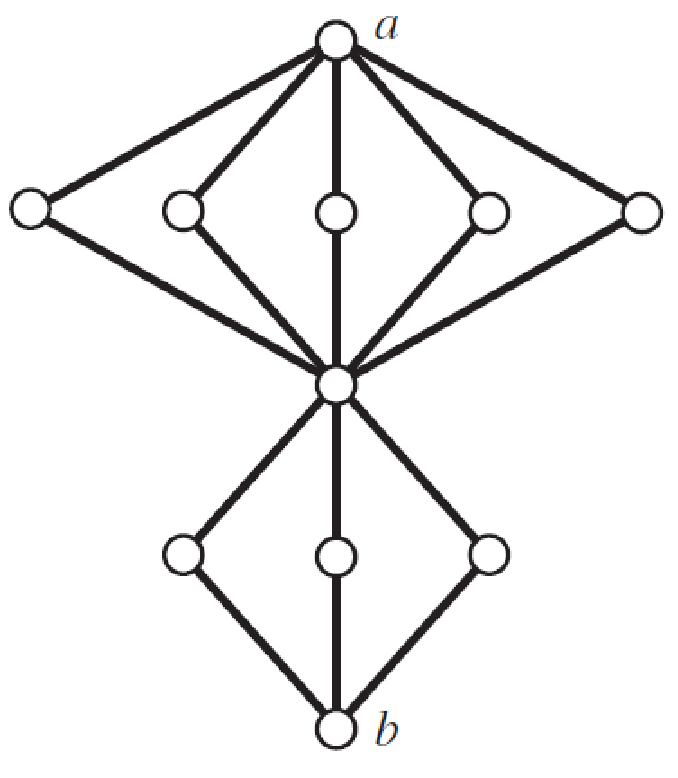
\includegraphics[scale=0.3]{WS1.pdf}
\end{figure}
\enumb
\item How many different paths are there from $a$ to $b$? $5\cdot 3=15$
\item How many different walks are there from $a$ to $b$? INFINITELY MANY
\enume
\item Prove that $K_n$ is connected.
\begin{proof}
Let $x,y\in V(K_n)$, then $xy\in E(K_n)$ and the path $P=x\sim y$ connects the two. Since the choice of $x$ and $y$ were arbitrary, this finishes the proof.
\end{proof}
\item Suppose $G$ is a connected graph in which each vertex has even degree. Then, $G$ has no cut edges.
\begin{proof}
FTSC assume that there there is a cut edge $e=xy$. Then $G-e$ has two components $G_1$ and $G_2$ with $x\in G_1$ and $y\in G_2$. Then removing $e$ decreases the degree of $x$ by one which now becomes an odd number. However, the degree of other vertices in $G_1$ are unaffected and thus
\[
\sum_{v\in V(G_1)}d_{G_1}(v) = \sum_{x\neq v\in V(G_1)}d_{G_1}(v)+d_{G_1}(x)
\]
which is the sum of an even and an odd number and therefore it is odd. However, this contradicts $G_1$ being a graph.
\end{proof}

\item List all the trees
\enumb
\item with vertex set $\{1,2,3\}$. The only one is $P_3$
\item with vertex set $\{1,2,3,4\}$. We have $P_4$ and the star.
\enume
\item 
\begin{enumerate}
\item[a)] Let $T$ be a tree with $n\geq 1$ vertices. Prove that $T$ has $n-1$ edges.

\begin{proof}
We prove this by induction. The base case checks out as $n=1$ is just one vertex with $1-1=0$ edges.

By the induction hypothesis, suppose the result is true for $n=k$ and let $T$ be a tree on $n=k+1$ vertices. Let $v$ be a leaf of $T$ and let $T'=T-v$. Then $T'$ is a tree with $k$ vertices and thus it has $k-1$ edges. Since $v$ is a leaf, $d(v)=1$ and therefore we only lost one edge by deleting it, that is $T$ has $k+1$ edges as required.
\end{proof}
\item[b)] Prove the converse, i.e. that if $G$ is a connected graph that has exactly $n-1$ edges then $G$ must be a tree.

\begin{proof}
Suppose $G$ is a connected graph with $n$ vertices and $n-1$ edges. We know that $G$ has a spanning tree $T$. However,
\[
|E(T)|=|V(T)|-1=|V(G)|-1=|E(G)|
\]
and it turns out that we did not throw out any edges. Therefore $G=T$ and thus it's a tree.
\end{proof}
\end{enumerate}

\item Let $T$ be a tree. Prove that the average degree of a vertex in $T$ is less than $2$.

\begin{proof}
\[
d_avg=\frac{1}{|V(G)|}\sum_{v\in V(G)}d_G(v)=2\frac{|E(G)|}{|V(G)|}=2\frac{n-1}{n}<2
\]
\end{proof}

\enume
\end{document}